\documentclass[eng,printmode,openright]{mgr} %openany openright
\usepackage[utf8x]{inputenc}
\usepackage{ucs}
\usepackage[MeX]{polski}
\usepackage{geometry}
\usepackage{subfigure}
\usepackage{fancyhdr}
\usepackage{amsmath}
\usepackage{amsfonts}
\usepackage{amssymb}
\usepackage{pdflscape}
\usepackage{float}
\pagestyle{fancy}
\usepackage{graphicx} 
\usepackage{graphicx}
\usepackage{subfigure}
\usepackage{psfrag}
%pakiety dodające dużo dodatkowych poleceń matematycznych
\usepackage{amsmath}
\usepackage{amsfonts}
%pakiety wspomagające i poprawiające składanie tabel
\usepackage{supertabular}
\usepackage{array}
\usepackage{tabularx}
\usepackage{hhline}
\usepackage{float}
\usepackage{indentfirst}
\usepackage{color}
\usepackage{enumerate}

\begin{document}

\newgeometry{tmargin=3cm, bmargin=3cm, lmargin=2cm, rmargin=2cm}
Autor: Radosław Taborski 209347 \hspace{10em} Termin: środa 12:50

\begin{center}
\huge{\textbf{Sprawozdanie z projektu specjalnościowego}}\\

\large{\textbf{dr inż. Krzysztof Halawa}}
\end{center}

\begin{enumerate}
	\item {\large \textbf{Cel}}
	
	Celem projektu jest wykonanie bazy danych, aplikacji zarządzającej bazą danych i aplikacji webowej rozszerzające system bezprzewodowego pomiaru temperatury.
	 
	 %TODO: poprawić schemat tak abyy opowiadał projektowi specjalnościowemu
	\begin{figure}[H]
		\centering
		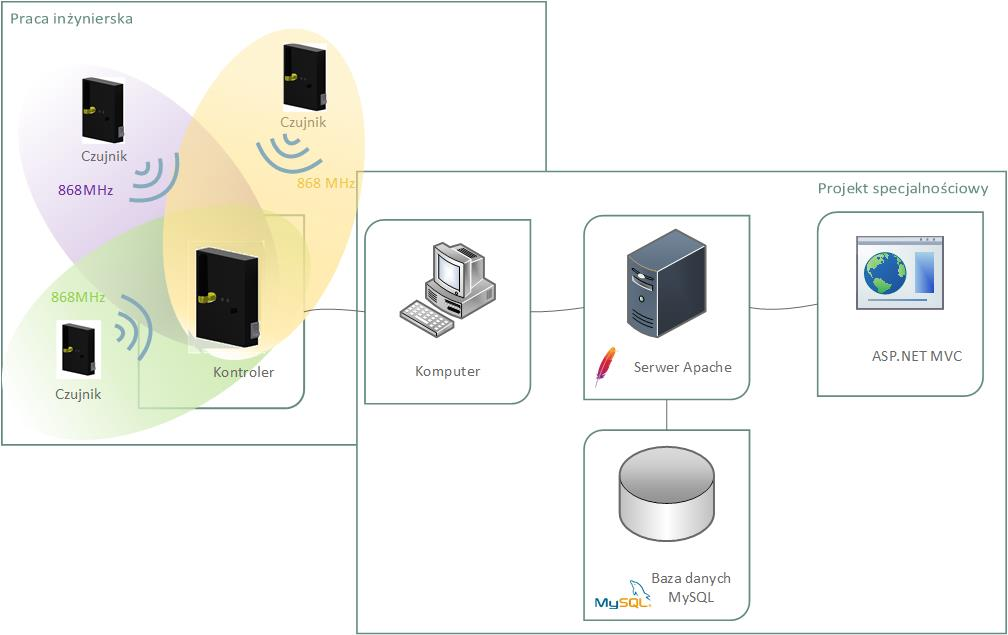
\includegraphics[width=1\linewidth]{schemat.jpg}
		\caption{Schemat systemu z podziałem na elementy wykonane w pracy inżynierskiej i projekcie specjalnościowym }
		\label{schemat}
	\end{figure}
	
	
	\item {\large \textbf{Wykonanie}}
	\begin{itemize}		
		\item \textbf{{\large Baza danych}}
		
		Stworzona została baza danych, która w prosty sposób przechowuje pomiary temperatur dla skonstruowanych w pracy inżynierskiej czujników. Baza danych dzięki aplikacji XAMPP została umieszczona na serwerze lokalnym. 
		
		\begin{figure}[H]
			\centering
			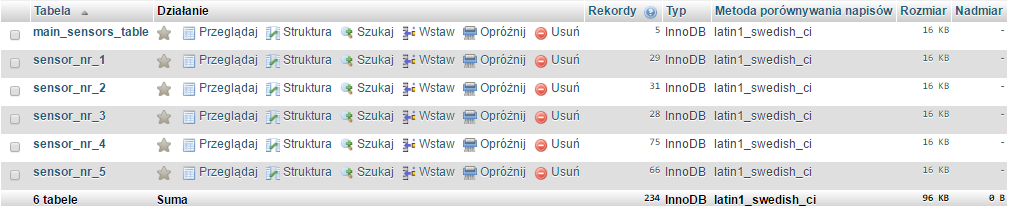
\includegraphics[width=1\linewidth]{BazaDanych1.png}
			\caption{Utworzone tabele}
			\label{tabele}
		\end{figure}
		
		Wykonana została jedna tabela główna, w której przechowywane są informacje takie jak nazwa czujnika, adres jaki ma przypisany w systemie oraz ostatnią temperaturę jaka została zmierzona.
		Na rysunkach \ref{model_fizyczny_main} i \ref{main_table} przedstawiony został model fizyczny oraz przykładowa zawartość tej tabeli. 
		
		\begin{figure}[H]
			\centering
			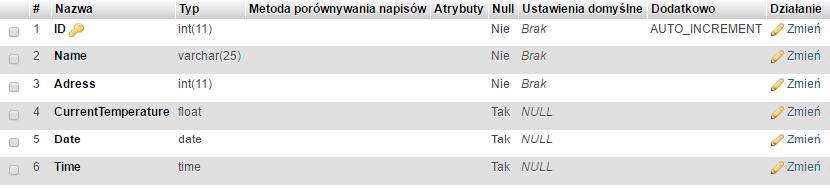
\includegraphics[width=1\linewidth]{BazaDanych5.png}
			\caption{Model fizyczny głównej tabeli}
			\label{model_fizyczny_main}
		\end{figure}			
		\begin{figure}[H]
			\centering
			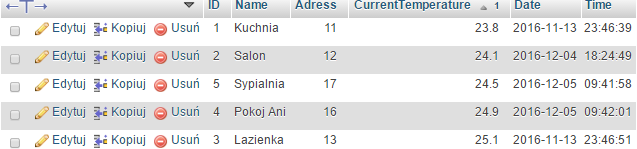
\includegraphics[width=1\linewidth]{BazaDanych2.png}
			\caption{Główna tabela z zapisanymi czujnikami}
			\label{main_table}
		\end{figure}
		
		Tabele dla poszczególnych czujników są tworzone dynamicznie w raz z dodawaniem nowego bezprzewodowego czujnika do sieci. Przechowywana w nich jest cała historia zmierzonych temperatur, wraz z datą ich pomiaru. Na rysunkach \ref{model_fizyczny_sensor} i \ref{sensor_table} pokazany został model tabeli dla konkretnego czujnika oraz przykładową zawartość.
		\begin{figure}[H]
			\centering
			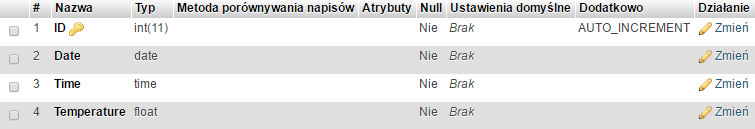
\includegraphics[width=1\linewidth]{BazaDanych4.png}
			\caption{Model fizyczny tabeli z pomiarami}
			\label{model_fizyczny_sensor}
		\end{figure}
		\begin{figure}[H]
			\centering
			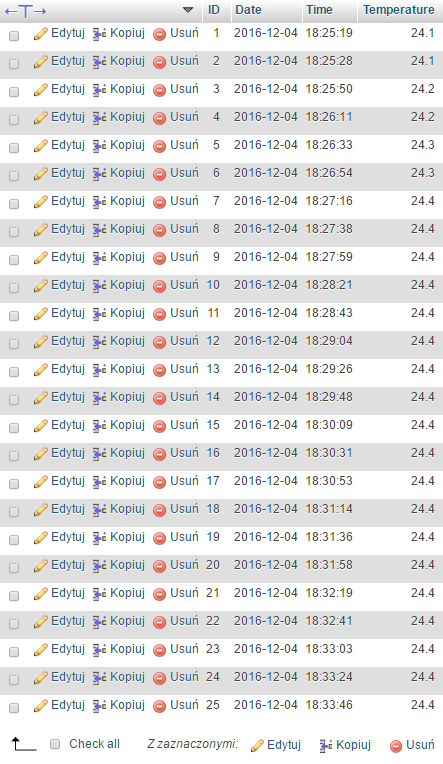
\includegraphics[width=0.6\linewidth]{BazaDanych3.png}
			\caption{Przykładowa tabela z pomiarami}
			\label{sensor_table}
		\end{figure}


		Baza danych złożona jest z jednej tabeli głównej oraz wielu innych tabel o identycznej strukturze pól. Każda tabela jest samodzielnym dokumentem i nie współpracuje z innymi tabelami. Jest to tzw. Kartotekowa baza danych.
		
		\begin{figure}[H]
			\centering
			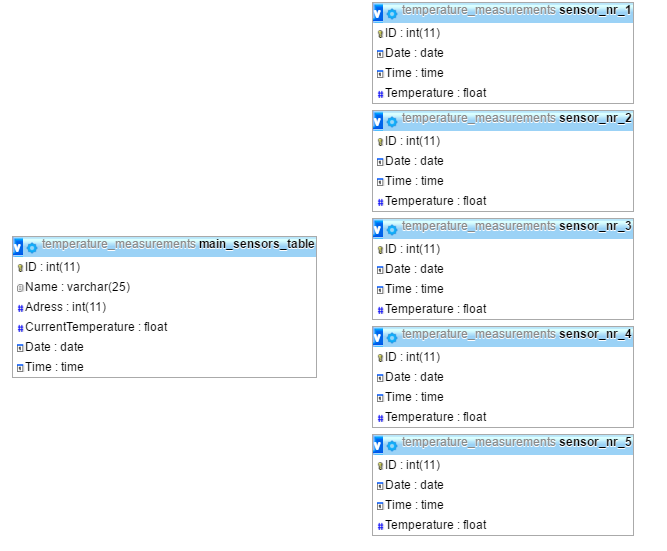
\includegraphics[width=0.8\linewidth]{BazaDanych6.png}
			\caption{Widok projektu bazy danych}
			\label{relacje}
		\end{figure}
			
		\item \textbf{{\large Aplikacja zarządzająca bazą danych}}
		
		Aplikacja ta odczytuje dane wysyłane do komputera standardem RS232 z wykorzystaniem złącza USB przez kontroler sieci bezprzewodowej. Jednak nim to następuje, pomyślnie zakończyć musi się szereg czynności takich jak: łączenie z serwerem, łączenie z bazą danych oraz przygotowanie do wymiany informacji poprzez port szeregowy.
		
		Parametry transmisji szeregowej:
		\begin{itemize}
			\item prędkość transmisji (baud rate): 2400 b/s
			\item 8 bitów danych
			\item brak bitu parzystości
			\item dwa bity stopu
		\end{itemize}
		
		Dodanie nowego czujnika do systemu powoduje zapytanie aplikacji o jego nazwę oraz po podaniu tej wartości dodanie rekordu do głównej tabeli z czujnikami. Utworzena również zostaje nowa tabela dla konkretnego czujnika, która przechowuje wszystkie pomiary wykonane przez dany czujnik, wraz z datami.
			\begin{figure}[H]
				\centering
				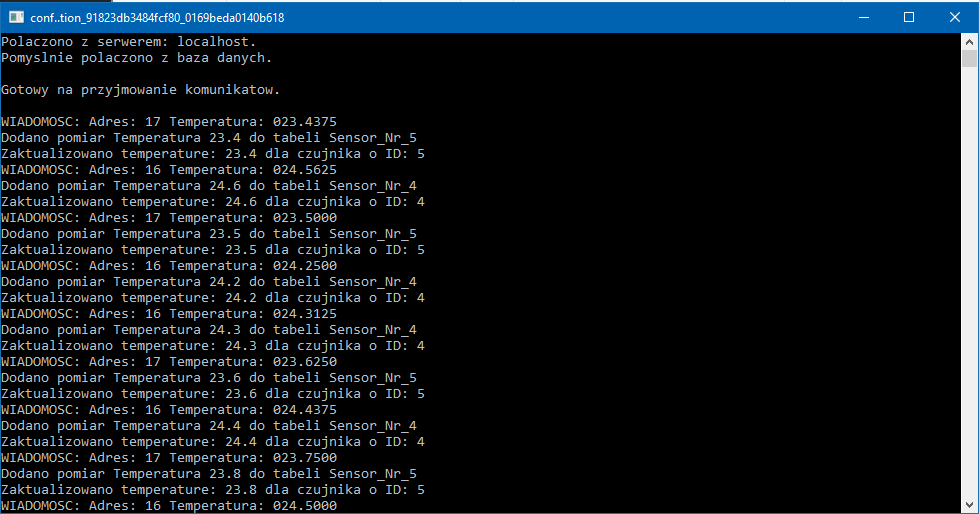
\includegraphics[width=1\linewidth]{Config.png}
				\caption{Wygląd aplikacji dodającej pomiary do bazy danych}
				\label{config}
			\end{figure}
		\item \textbf{{\large Aplikacja webowa}}
		
		 Do budowy aplikacji webowej została użyta platforma aplikacyjna ASP.NET z wykorzystaniem wzorca MVC, w zintegrowanym środowisku programistycznym Microsoft Visual Studio. Aplikacja webowa służy do wizualizowania danych zapisanych w bazie danych. Umożliwia śledzenie aktualnych temperatur w pomieszczeniach w czasie rzeczywistym oraz przeanalizowanie historii pomiarów z konkretnego pomieszczenia i z konkretnego dnia lub całego okresu pomiarowego.
		 \begin{figure}[H]
		 	\centering
		 	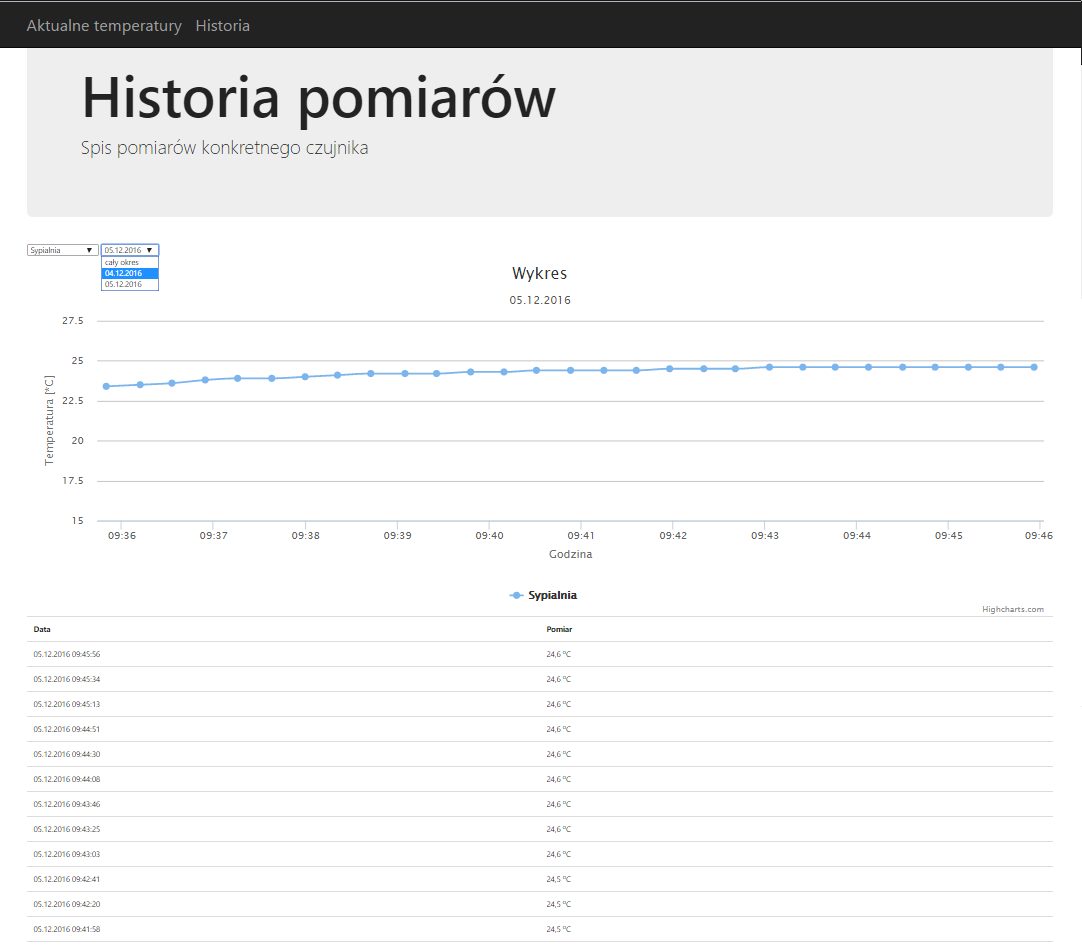
\includegraphics[width=1\linewidth]{Historia.png}
		 	\caption{Wygląd strony ze statystykami i historią pomiarów}
		 	\label{web_history}
		 \end{figure}
		 
		\begin{figure}[H]
			\centering
			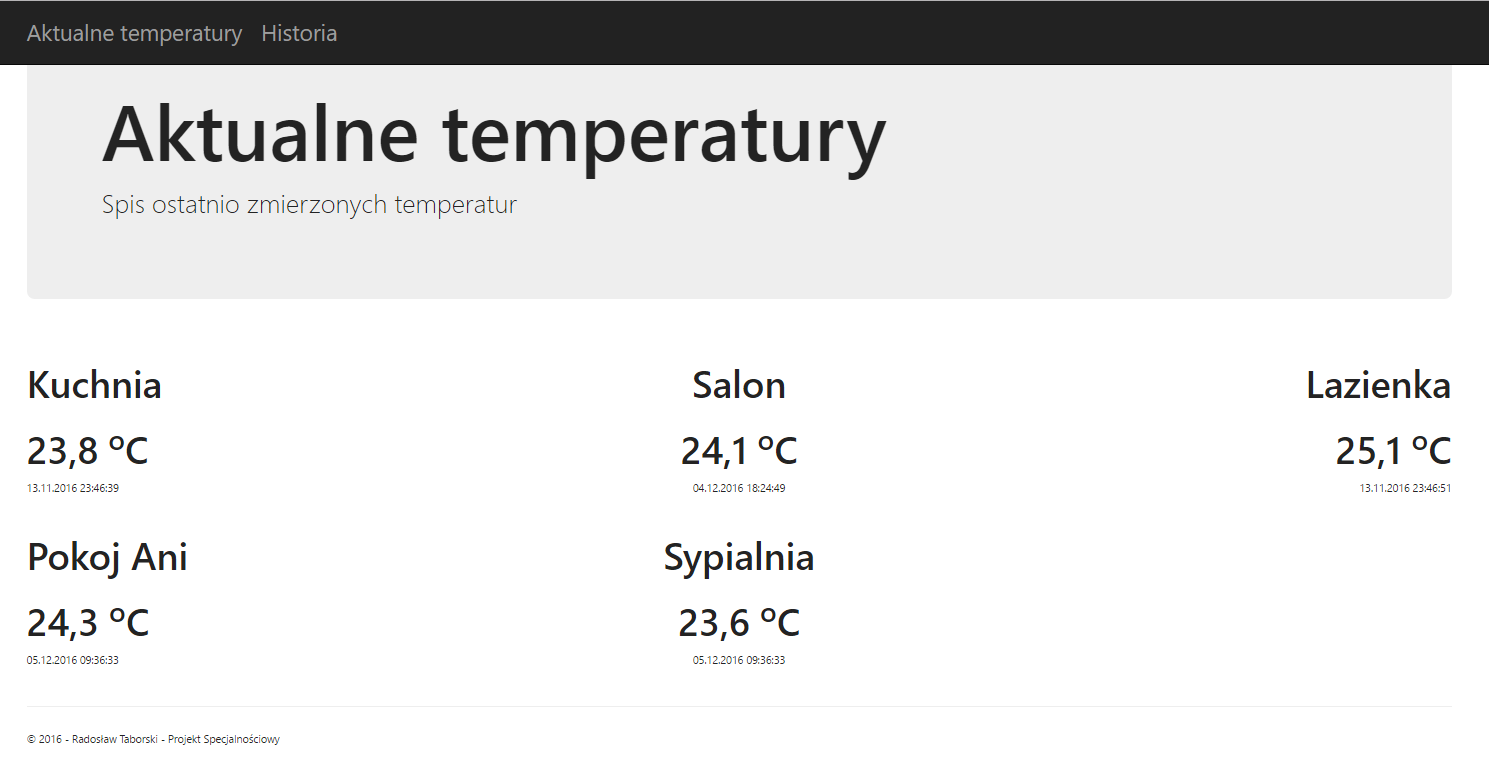
\includegraphics[width=1\linewidth]{Aktualne.png}
			\caption{Wygląd głównej strony z aktualnymi temperaturami w pomieszczeniach}
			\label{web_actually}
		\end{figure}
		
	\end{itemize}
	
	\item {\large \textbf{Podsumowanie}}
	
	Stworzone funkcjonalności zostały przetestowane wraz z wykonanymi w pracy inżynierskiej czujnikami. 
	Współpraca wszystkich aplikacji ze sobą oraz z projektem inżynierskim działa bez zarzutu.
\end{enumerate}

\end{document}